\documentclass[12pt, twoside]{report} % basis ukuran font adalah 12 poin dan opsi twoside untuk keperluan penomoran halaman kiri-kanan

% spesifikasi kertas, margin, font, line spacing, dan footer
\usepackage[paper = a4paper,
            left = 3cm, 
            right = 3cm, 
            top = 3cm, 
            bottom = 3cm]{geometry}

\usepackage[indonesian]{babel} % agar pemenggalan kata sesuai kbbi
\usepackage[utf8]{inputenc}

% pengaturan auto text pada footer
\usepackage{fancyhdr}
\pagestyle{fancy}
\fancyhead{} % hapus semua header
\fancyfoot{} % hapus semua footer
% hilangkan garis dan jarak pada header
\renewcommand{\headrulewidth}{0pt}
\renewcommand{\headruleskip}{0pt}
% hilangkan garis dan jarak pada footer
\renewcommand{\footrulewidth}{0pt}
\renewcommand{\footruleskip}{0pt}
\usepackage{helvet} % font arial
\fancyfoot[R]{\sffamily \small \textbf{Universitas Indonesia}} % digunakan font arial yang di-bold dengan ukuran small agar ukuran font menjadi 10 poin karena basis ukuran font adalah 12 poin

\usepackage{mathptmx} % font times new roman

\usepackage{setspace}
\onehalfspacing % line spacing = 1.5 lines

% mengganti judul table of contents, list of tables, list of figures, bab, dan bibliography, serta nama gambar dan tabel ke Bahasa Indonesia
\addto\captionsindonesian{\renewcommand{\contentsname}{DAFTAR ISI}}
\addto\captionsindonesian{\renewcommand{\listfigurename}{DAFTAR GAMBAR}}
\addto\captionsindonesian{\renewcommand{\listtablename}{DAFTAR TABEL}}
\addto\captionsindonesian{\renewcommand{\chaptername}{BAB}}
\addto\captionsindonesian{\renewcommand{\bibname}{DAFTAR REFERENSI}}

\def\figurename{Gambar}
\def\tablename{Tabel}

% perintah baru untuk memasukkan judul chapter yang bukan bab ke daftar isi
\newcommand{\addchapter}[1]{
    \addcontentsline{toc}{chapter}{#1}
}

\setcounter{secnumdepth}{3} % maksimum hanya sampai subsubsection 
\setcounter{tocdepth}{3} % menampilkan sampai subsubsection pada daftar isi

% pengaturan tampilan bab
\usepackage{sectsty}
\usepackage{titlesec}
\sectionfont{\normalsize} % ukuran font section adalah 12 poin
\subsectionfont{\normalsize} % ukuran font subsection adalah 12 poin
\titleformat{\chapter}[display]   
{\centering \normalsize \bfseries}{\chaptertitlename\ \thechapter}{0pt}{\normalsize}   
\titlespacing*{\chapter}{0pt}{-20pt}{20pt}

% hal-hal yang berkaitan dengan matematika (salinan dari templat latex proposal skripsi dengan sedikit modifikasi)
\usepackage{amsmath, amssymb, amsthm}
\numberwithin{equation}{chapter}

\theoremstyle{definition} % Isi teorema tidak ditulis miring
\newtheorem{theorem}{Teorema}[chapter]
\newtheorem{lemma}[theorem]{Lema} 
\newtheorem{proposition}[theorem]{Proposisi}
\newtheorem{corollary}[theorem]{Akibat}
\newtheorem{definition}{Definisi}[chapter]
\newtheorem{example}{Contoh}[chapter]
\newtheorem*{remark}{Catatan}
\def\proofname{Bukti}

% hapus jarak pemisah untuk enumerate dan itemize agar jarak konsisten
\usepackage{enumitem}
\setlist[enumerate]{nosep}
\setlist[itemize]{nosep}

% mengatur jarak antara gambar dan caption gambar agar konsisten dengan line spacing yang digunakan
\usepackage[skip = 8pt]{caption}
\raggedbottom

% pengaturan daftar referensi
\usepackage[natbibapa]{apacite}
\bibliographystyle{apacite}
\renewcommand{\BOthers}{dkk} % mengubah et al. menjadi dkk.
\renewcommand{\BBAB}{dan} % mengubah kata and dalam sitasi in-text (\citet) menjadi &
\renewcommand{\BRetrievedFrom}{} % menghilangkan frasa "retrieved from"
\renewcommand{\doiprefix}{} % menghilangkan kata "doi:"

\usepackage{url}
\AtBeginDocument{\urlstyle{APACsame}} % agar font tautan yang ditampilkan sama dengan font yang digunakan dalam keseluruhan dokumen

% pengaturan lampiran
\usepackage{tocloft}
\newcommand{\listappendicesname}{DAFTAR LAMPIRAN}
\newlistof{appendices}{apc}{\listappendicesname}
\newcommand{\appendices}[1]{\addcontentsline{apc}{appendices}{#1}}
\newcommand{\newappendix}[1]{\section*{#1}\appendices{#1}}
\renewcommand{\cftapctitlefont}{\hfill\normalsize\bfseries} 
\renewcommand{\cftafterapctitle}{\hfill}
\addtolength{\cftbeforeapctitleskip}{-2.25cm} % jarak sebelum judul daftar lampiran
\addtolength{\cftafterapctitleskip}{0cm} % jarak setelah judul daftar lampiran

% pengaturan ulang tampilan judul daftar isi, daftar gambar, dan daftar tabel akibat penggunaan package tocloft
\renewcommand{\cfttoctitlefont}{\hfill\normalsize\bfseries}
\renewcommand{\cftaftertoctitle}{\hfill}
\addtolength{\cftbeforetoctitleskip}{-2.25cm} % jarak sebelum judul daftar isi
\addtolength{\cftaftertoctitleskip}{0cm} % jarak setelah judul daftar isi

\renewcommand{\cftloftitlefont}{\hfill\normalsize\bfseries}
\renewcommand{\cftafterloftitle}{\hfill}
\addtolength{\cftbeforeloftitleskip}{-2.25cm} % jarak sebelum judul daftar gambar
\addtolength{\cftafterloftitleskip}{0cm} % jarak setelah judul daftar gambar

\renewcommand{\cftlottitlefont}{\hfill\normalsize\bfseries}
\renewcommand{\cftafterlottitle}{\hfill}
\addtolength{\cftbeforelottitleskip}{-2.25cm} % jarak sebelum judul daftar tabel
\addtolength{\cftafterlottitleskip}{0cm} % jarak setelah judul daftar tabel

% package lain yang diperlukan (tambahkan package yang diperlukan)
\usepackage{array}
\usepackage{emptypage}
\usepackage{float}
\usepackage{graphicx}
\usepackage{hyperref}
\usepackage{indentfirst}
\usepackage{lipsum}
\usepackage{tabularx}


%----------memulai dokumen----------
\begin{document}

% ganti isi dalam kurung kurawal kedua sesuai data diri dan tugas akhir Anda

\newcommand{\judul}{Rute Optimal untuk Mendapatkan Jumat Berkah dengan Menggunakan Algoritma X}

\newcommand{\titles}{The Optimal Route to Get a Friday Berkah Using X Algorithm} % judul dalam bahasa Inggris

\newcommand{\jenis}{Skripsi}

\newcommand{\nama}{Jono D. Joestar}

\newcommand{\npm}{2169420666}

\newcommand{\fakultas}{Matematika dan Ilmu Pengetahuan Alam}

\newcommand{\prodi}{Sarjana Matematika}

\newcommand{\programme}{Undergraduate Programme in Mathematics} % prodi dalam bahasa Inggris

\newcommand{\gelar}{Sarjana Sains}

\newcommand{\tempat}{Depok}

\newcommand{\tanggal}{15}

\newcommand{\bulan}{Juni}

\newcommand{\tahun}{2025}

% halaman sampul dan judul menggunakan line spacing = single
\begin{singlespace}
%----------Halaman Sampul----------
\begin{titlepage}
    \begin{center}
        
\includegraphics[width=3cm]{gambar/logo ui hitam.png}
        
        \bfseries
        UNIVERSITAS INDONESIA

        \vspace{1cm}
        \large 
        \MakeUppercase{\judul}

        \vspace{4cm}
        
        \MakeUppercase{\jenis}

        \vspace{4cm}
        \normalsize
        \MakeUppercase{\nama}\\
        \npm

        \vspace{5cm}
        FAKULTAS \MakeUppercase{\fakultas}\\
        PROGRAM STUDI \MakeUppercase{\prodi}\\
        \MakeUppercase{\tempat}\\
        \MakeUppercase{\bulan} \tahun
    \end{center}
    \normalfont
\end{titlepage}

\newpage

\pagenumbering{roman} % mulai dari halaman judul digunakan penomoran halaman dengan angka romawi kecil, tetapi khusus halaman judul, nomor halamannya tidak ditampilkan

%----------Halaman Judul----------
\addchapter{HALAMAN JUDUL}
\begin{titlepage}
    \begin{center}
        
\includegraphics[width=3cm]{gambar/logo ui hitam.png}
        
        \bfseries
        UNIVERSITAS INDONESIA

        \vspace{1cm}
        \large
        \MakeUppercase{\judul}

        \vspace{4cm}
        
        \MakeUppercase{\jenis}\\

        \normalsize
        Diajukan sebagai salah satu syarat untuk memperoleh gelar \gelar

        \vspace{4cm}
        
        \MakeUppercase{\nama}\\
        \npm

        \vspace{5cm}
        FAKULTAS \MakeUppercase{\fakultas}\\
        PROGRAM STUDI \MakeUppercase{\prodi}\\
        \MakeUppercase{\tempat}\\
        \MakeUppercase{\bulan} \tahun
    \end{center}
    \normalfont
\end{titlepage}
\end{singlespace}

\newpage

% style halaman sebelum abstrak: hanya ada nomor halaman di tengah bawah
\setcounter{page}{2}
\fancypagestyle{plain}{
    \fancyhead{} % hapus semua header
    \fancyfoot{} % hapus semua footer
    \fancyfoot[C]{\thepage} % posisikan nomor halaman di tengah bawah
}

%----------Halaman Pernyataan Orisinalitas----------
\addchapter{HALAMAN PERNYATAAN ORISINALITAS}
% halaman pernyataan orisinalitas menggunakan line spacing = double
\begin{doublespace}
\chapter*{HALAMAN PERNYATAAN ORISINALITAS}

\centering
\vspace{1.5cm}
\jenis \,\ ini adalah hasil karya saya sendiri,\\
dan semua sumber baik yang dikutip maupun dirujuk\\
telah saya nyatakan benar.

\vspace{3cm}
\begin{tabular}{@{}ll}
     Nama           &: \nama\\
     NPM            &: \npm\\
     Tanda Tangan   &: \\[1.5cm]
     Tanggal        &: \tanggal \,\ \bulan \,\ \tahun
\end{tabular}

\end{doublespace}

\newpage

%----------Halaman Pengesahan----------
\addchapter{HALAMAN PENGESAHAN}
% halaman pengesahan menggunakan line spacing = single
\begin{singlespace}
    \chapter*{HALAMAN PENGESAHAN}

\vspace{0.5cm}
\noindent
\begin{tabularx}{\textwidth}{@{}l@{\hspace{1em}}lX@{}}
\jenis \,\ ini diajukan oleh & : & \\
Nama                     & : & \nama\\
NPM                      & : & \npm\\
Program Studi            & : & \prodi\\
Judul \jenis             & : & \judul
\end{tabularx}

\vspace{1.25cm}
\noindent
Telah berhasil dipertahankan di hadapan Dewan Penguji dan diterima sebagai bagian persyaratan yang diperlukan untuk memperoleh gelar \gelar \,\ pada Program Studi \prodi, Fakultas \fakultas, Universitas Indonesia.

\vspace{1cm}
\begin{center}
    \textbf{DEWAN PENGUJI}
\end{center}

\vspace{0.5cm}
\noindent
% ini untuk S-1/ S-2
\begin{tabularx}{\textwidth}{@{}l@{\hspace{1em}}l@{\hspace{1em}}lX@{}}
Pembimbing I    & : & Dr. Fulan & $\Biggl(\hspace{3cm}\Biggl)$\\[1cm]
Pembimbing II   & : & Fulana, S.Si., M.Si., Ph.D.  & $\Biggl(\hspace{3cm}\Biggl)$\\[1cm]
Penguji I       & : & Dr. Fulani, S.Si., M.T. & $\Biggl(\hspace{3cm}\Biggl)$\\[1cm]
Penguji II      & : & Dra. Fulano, M.Kom, Ph.D. & $\Biggl(\hspace{3cm}\Biggl)$
\end{tabularx}
% ini untuk S-3 (hapus bagian untuk S-1/S-2 dan tanda persen dari setiap baris berikut jika Anda adalah mahasiswa S-3)
%\begin{tabularx}{\textwidth}{@{}l@{\hspace{1em}}l@{\hspace{1em}}l@{\hspace{1em}}lX@{}}
%Promotor     & : & Dr. Fulan &   & $\biggl(\hspace{3cm}\biggl)$\\[0.5cm]
%Kopromotor   & : & Fulana, S.Si., M.Si., Ph.D.  &   & $\biggl(\hspace{3cm}\biggl)$\\[0.5cm]
%             & : & Fulana, S.Si., M.Si., Ph.D.  &   & $\biggl(\hspace{3cm}\biggl)$\\[0.5cm]
%Tim Penguji  & : & Dr. Fulani, S.Si., M.T. & (Ketua) & $\biggl(\hspace{3cm}\biggl)$\\[0.5cm]
%             & : & Dra. Fulano, M.Kom, Ph.D. & (Anggota) & $\biggl(\hspace{3cm}\biggl)$\\[0.5cm]
%             & : & Dra. Fulano, M.Kom, Ph.D. & (Anggota) & $\biggl(\hspace{3cm}\biggl)$\\[0.5cm]
%             & : & Dra. Fulano, M.Kom, Ph.D. & (Anggota) & $\biggl(\hspace{3cm}\biggl)$   
%\end{tabularx}

\vspace{2.5cm}
\noindent
\begin{tabularx}{\textwidth}{@{}l@{\hspace{1em}}lX@{}}
Ditetapkan di & : & \tempat\\
Tanggal       & : & \tanggal \,\ \bulan \,\ \tahun
\end{tabularx}
\end{singlespace}

\newpage

%----------Kata Pengantar----------
\addchapter{KATA PENGANTAR}
\chapter*{KATA PENGANTAR}

\vspace{28pt} % jarak judul ke isi kata pengantar adalah 2x2 spasi
\noindent
\lipsum[1]

\begin{flushright}
    \begin{tabular}{@{}c@{}}
     \nama\\
     \vspace{0.25cm}\\
     \tahun
\end{tabular}
\end{flushright}

\newpage

%----------Halaman Pernyataan Persetujuan Publikasi Tugas Akhir untuk Kepentingan Akademis----------
\addchapter{HALAMAN PERNYATAAN PERSETUJUAN PUBLIKASI TUGAS AKHIR UNTUK KEPENTINGAN AKADEMIS}
\begin{singlespace} % khusus judul menggunakan line spacing = single
\chapter*{HALAMAN PERNYATAAN PERSETUJUAN PUBLIKASI TUGAS AKHIR UNTUK KEPENTINGAN AKADEMIS}
\end{singlespace}
\vspace{-0.65cm}
\par\noindent\rule{\textwidth}{3pt}
\par
\vspace{0.35cm}
\noindent
Sebagai sivitas akademik Universitas Indonesia, saya yang bertanda tangan di bawah ini:

\vspace{0.5cm}
\noindent
\begin{tabular}{@{}m{3cm} m{10cm}}
    Nama            &: \nama\\
    NPM             &: \npm\\
    Program Studi   &: \prodi\\
    Fakultas        &: \fakultas\\
    Jenis Karya     &: \jenis
\end{tabular}

\vspace{0.5cm}
\noindent 
demi pengembangan ilmu pengetahuan, menyetujui untuk memberikan kepada Universitas Indonesia \textbf{Hak Bebas Royalti Noneksklusif (\textit{Non-exclusive Royalty-Free Right})} atas karya ilmiah saya yang berjudul:

\vspace{0.5cm}
\begin{center}
    \judul
\end{center}
beserta perangkat yang ada (jika diperlukan). Dengan Hak Bebas Royalti Noneksklusif ini Universitas Indonesia berhak menyimpan, mengalihmediakan/mengalihformatkan, mengelola dalam bentuk pangkalan data (\textit{database}), merawat, dan memublikasikan tugas akhir saya selama tetap mencantumkan nama saya sebagai penulis/pencipta dan sebagai pemilik Hak Cipta. 


\vspace{0.5cm}
\noindent 
Demikian pernyataan ini saya buat dengan sebenarnya.
\begin{center}
    \begin{tabular}{@{}rm{3cm} lm{10cm}}
        Dibuat di     &: \tempat\\
        Pada Tanggal  &: \tanggal \,\ \bulan \,\ \tahun
    \end{tabular}

    \vspace{0.2cm}
    Yang menyatakan

    \vspace{2cm}
    (\nama)
\end{center}

\newpage

% style untuk setiap awal bab
\fancypagestyle{plain}{
    \fancyhead{} % hapus semua header
    \fancyfoot{} % hapus semua footer
    \fancyfoot[C]{\thepage} % posisikan nomor halaman di tengah bawah
    \fancyfoot[R]{\sffamily \small \textbf{Universitas Indonesia}} % digunakan font arial yang di-bold dengan ukuran small agar ukuran font menjadi 10 poin karena basis ukuran font adalah 12 poin
}

%----------Abstrak----------
\addchapter{ABSTRAK}
\chapter*{ABSTRAK}

\noindent
\begin{tabularx}{\textwidth}{@{}l@{\hspace{1em}}lX@{}}
Nama                     & : & \nama\\
Program Studi            & : & \prodi\\
Judul \jenis             & : & \judul
\end{tabularx}

\vspace{0.5cm}
\noindent
\lipsum[1] (Maksimum 500 kata dan hanya dalam 1 paragraf)

\vspace{0.5cm}
\noindent
Kata kunci:\\
minimal 3 kata.

\newpage

%----------Abstract----------
\addchapter{ABSTRACT}
\chapter*{ABSTRACT}

\noindent
\begin{tabularx}{\textwidth}{@{}l@{\hspace{1em}}lX@{}}
Name                     & : & \nama\\
Program                  & : & \programme\\
Title                    & : & \titles
\end{tabularx}

\vspace{0.5cm}
\noindent
\lipsum[1] (Maximum 500 words and only in 1 paragraph)

\vspace{0.5cm}
\noindent
Keywords:\\
minimum 3 words.

\newpage

% daftar isi, daftar gambar, dan daftar tabel menggunakan line spacing = single
\begin{singlespace}
%----------Daftar Isi----------
\addchapter{DAFTAR ISI}
\pagestyle{plain}
\tableofcontents

\newpage

%=====Hapus bagian ini jika tidak ada gambar dalam tugas akhir Anda (dari sini)=====
%----------Daftar Gambar----------
\addchapter{DAFTAR GAMBAR}
\listoffigures

\newpage
%=====(sampai sini)=====


%=====Hapus bagian ini jika tidak ada tabel dalam tugas akhir Anda (dari sini)=====
%----------Daftar Tabel----------
\addchapter{DAFTAR TABEL}
\listoftables

\newpage
%=====(sampai sini)=====


%=====Hapus bagian ini jika tidak ada lampiran dalam tugas akhir Anda (dari sini)=====
%----------Daftar Lampiran----------
\addchapter{DAFTAR LAMPIRAN}
\listofappendices
%=====(sampai sini)=====

\end{singlespace}

\cleardoublepage

% style penomoran halaman bagian isi
\fancyhead[LE, RO]{\thepage}
\pagenumbering{arabic}

%----------BAB 1----------
\chapter{PENDAHULUAN}

\section{Latar Belakang}
\lipsum[1-4]

\section{Rumusan Masalah}
Lorem ipsum dolor sit amet, consectetuer adipiscing elit. Ut purus elit, vestibulum
ut, placerat ac, adipiscing vitae, felis.
\begin{enumerate}
    \item tes1?
    \item tes2?
    \item tes3?
\end{enumerate}
Mantap, jaraknya konsisten.

\section{Tujuan Penelitian}
Lorem ipsum dolor sit amet, consectetuer adipiscing elit. Ut purus elit, vestibulum
ut, placerat ac, adipiscing vitae, felis.
\begin{enumerate}
    \item tes1.
    \item tes2.
    \item tes3.
\end{enumerate}

\section{Batasan Penelitian} % kalau ada
Lorem ipsum dolor sit amet, consectetuer adipiscing elit. Ut purus elit, vestibulum
ut, placerat ac, adipiscing vitae, felis.
\begin{enumerate}
    \item tes1.
    \item tes2.
    \item tes3.
\end{enumerate}

\section{Metodologi Penelitian}
Lorem ipsum dolor sit amet, consectetuer adipiscing elit. Ut purus elit, vestibulum
ut, placerat ac, adipiscing vitae, felis.
\cleardoublepage

%----------BAB 2----------
\chapter{TINJAUAN PUSTAKA}

\section{Subbab Derajat Pertama}
Gunakan \texttt{$\backslash$citet\{\}} untuk melakukan kutipan dengan nama penulis disebutkan dalam kalimat. Contoh: \citet{knuth:1984} berpendapat bahwa .... 

Gunakan \texttt{$\backslash$citep\{\}} untuk melakukan kutipan dengan nama penulis tidak disebutkan dalam kalimat. Contoh: \LaTeX \, adalah ... \citep{latex:companion}. Perhatikan bahwa jika banyak penulis antara 3 sampai 5 orang, maka saat sitasi pertama kali semua penulis dituliskan. Namun, untuk selanjutnya akan ditulis 1 nama penulis pertama
dilanjutkan dengan "dkk" seperti ini \citep{latex:companion}.

\begin{equation}
    e^{i\pi}+1=0.
    \label{eq:euler}
\end{equation}
Persamaan \eqref{eq:euler} merupakan salah satu persamaan matematika terindah yang pernah saya lihat.

Vektor merupakan anggota ruang vektor. Definisi ruang vektor sebagai berikut.
\begin{definition}
    Himpunan tak-kosong $V$ disebut ruang vektor jika ....
    \label{def:ruangvektor}
\end{definition}
Berdasarkan Definisi \ref{def:ruangvektor}, kita dapat mengetahui bahwa suatu ....
Berikut ini adalah contoh ruang vektor riil.
\begin{example}
    Himpunan $C[0,1] = \{f:[0,1] \to \mathbb{R}\} | f \mbox{kontinu}$ merupakan ruang vektor.
\end{example}

Ruang vektor mempunyai sifat sebagai berikut.
\begin{theorem}
    Diberikan ruang vektor $V$ dan subruang $W$ dari $V$. Ruang vektor $V$ dapat ditulis sebagai
	\begin{equation}
		V = W \oplus W^{\perp}. \label{eq:dekomposisiruangvektor}
	\end{equation}
    \label{thm:gramschmidt}
\end{theorem}

\begin{proof}
    \lipsum[1]
\end{proof}

Berdasarkan Teorema \ref{thm:gramschmidt}, persamaan \eqref{eq:dekomposisiruangvektor} berguna dalam proses Gram-Schimdt.

\begin{lemma}
    Elemen nol pada grup $G$ bersifat tunggal.
\end{lemma}

\begin{corollary}
    Dekomposisi ruang vektor bersifat unik jika ...
\end{corollary}

\begin{remark}
    Lorem ipsum dolor sit amet, consectetuer adipiscing elit.
\end{remark}

\begin{figure}[H]
    \centering
    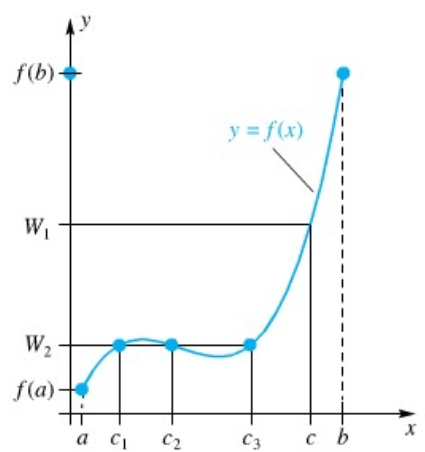
\includegraphics[width=0.5\linewidth]{gambar/teo_nilai_antara.png}
    \caption{Ilustrasi Teorema Nilai Antara}
    \caption*{\small \citep{varberg2007calculus}} % sumber gambar ditulis seperti ini jika gambar bukan buatan Anda sendiri
    \label{fig:teonilaiantara}
\end{figure}

Tambahkan ", telah diolah kembali" setelah sitasi sumber jika Anda sedikit menambahkan/memodifikasi gambar dari sumber yang Anda dapatkan. Misalkan gambar pada halaman selanjutnya sudah saya modifikasi.
\begin{figure}[H]
    \centering
    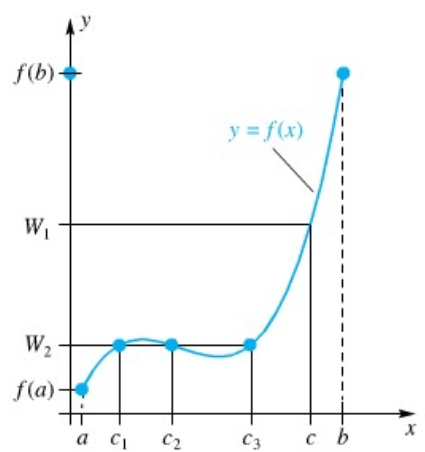
\includegraphics[width=0.5\linewidth]{gambar/teo_nilai_antara.png}
    \caption{Ilustrasi Teorema Nilai Antara 2}
    \caption*{\small \citep{varberg2007calculus}, telah diolah kembali} % sumber gambar ditulis seperti ini jika gambar bukan buatan Anda sendiri
    \label{fig:teonilaiantara2}
\end{figure}

Berikut adalah contoh tabel dalam \LaTeX.
\begin{table}[H]
    \centering
    \caption{Contoh Tabel 1}
    \begin{tabular}{|c|c|}
        \hline
        1 & 2 \\
        \hline
        3 & 4\\
        \hline
    \end{tabular}
    \label{tab:my_table}
\end{table}

\begin{table}[H]
    \centering
    \caption{Contoh Tabel 2}
    \begin{tabular}{ |c|c|c| } 
        \hline
        cell1 & cell2 & cell3 \\ 
        \hline
        cell4 & cell5 & cell6 \\ 
        cell7 & cell8 & cell9 \\ 
        \hline
    \end{tabular}
    \label{tab:my_label2}
\end{table}

\begin{remark}
    Ingat bahwa \textit{caption} serta sumber untuk gambar berada di bawah gambar, sedangkan untuk tabel berada di atas tabel.
\end{remark}
\subsection{Subbab Derajat Kedua}
\lipsum[1]

\subsubsection{Subbab Derajat Ketiga}
\lipsum[1]
\cleardoublepage

%----------BAB 3----------
\chapter{ANALISIS}

\section{Subbab Derajat Pertama}
\lipsum[1-5]

\subsection{Subbab Derajat Kedua}
\lipsum[1]

\subsection{Subbab Derajat Ketiga}
\lipsum[1]
\cleardoublepage

%----------BAB 4----------
\chapter{PENUTUP}

\section{Kesimpulan}
\lipsum[1]

\section{Saran}
\lipsum[1]
\cleardoublepage

%----------Daftar Referensi----------
\addchapter{DAFTAR REFERENSI}
\bibliography{referensi}

%----------Lampiran----------
%=====Hapus bagian ini jika tidak ada lampiran dalam tugas akhir Anda (dari sini)=====
\newpage
\makeatletter
\renewcommand\section{\@startsection {section}{1}{\z@}%
  {-3.5ex \@plus -1ex \@minus -.2ex}%
  {2.3ex \@plus.2ex}%
  {\raggedleft\normalsize}}
\makeatother

% untuk membuat judul lampiran, gunakan perintah (command) \newappendix
% catatan: jika suatu Lampiran n (n = 1, 2, 3, ...) lebih dari 1 halaman, maka buat seperti berikut.
% 1. potong bagian Lampiran n yang berada di halaman kedua.
% 2. buat halaman baru (\newpage) dan tempatkan bagian yang dipotong tadi di halaman baru tersebut. 
% 3. pada halaman baru untuk sambungan tersebut, tambahkan perintah (command): \section*{Lampiran n. Judul Lampiran n (lanjutan)} di atas isi lampiran yang dipotong tadi.

\newappendix{Lampiran 1. Lorem Ipsum}
\lipsum[1-4]
\newpage

\section*{Lampiran 1. Lorem Ipsum (lanjutan)}
\lipsum[5-6]
\newpage

\newappendix{Lampiran 2. Lorem Ipsum} \lipsum[1]
\newpage

\newappendix{Lampiran 3. Lorem Ipsum}
\lipsum[1]
%=====(sampai sini)=====

\end{document}
